\documentclass[10pt]{report}

\usepackage{float}
\usepackage{wrapfig}
\usepackage{graphicx}
\usepackage{color}
%\usepackage{epstopdf}
\usepackage{changepage}
\usepackage{amssymb}
\usepackage{amsthm}
\usepackage{amsmath}
\usepackage{booktabs}
\usepackage{listings}   % Include code snippets
\usepackage{titlesec}
\usepackage{ulem}
\usepackage{hyperref}
\usepackage{setspace}
\pdfpagewidth 8.5in
\pdfpageheight 11in
\topmargin -1.1in
\headheight 77pt
\headsep 0in
\textheight 8.5in
\textwidth 6.5in
\oddsidemargin 0in
\evensidemargin 0in
\footskip .4in
\definecolor{args}{rgb}{0.0,0.05,.33}
\definecolor{mygray}{rgb}{0.5,0.5,0.6}
\definecolor{mylightblue}{rgb}{.95, .95, .97}
\definecolor{mylightgreen}{rgb}{.95, .98, .95}
\definecolor{mymauve}{rgb}{0.58,0,0.82}
\lstset{language=Python, showstringspaces=false, frame=single, basicstyle=\footnotesize\sffamily, stringstyle=\color{mymauve}, framesep=4pt, xleftmargin=10pt, xrightmargin=10pt, rulecolor=\color{mygray}, backgroundcolor=\color{mylightgreen}, commentstyle=\color{mygray}, belowskip=2.5em, aboveskip=1em}

\lstdefinestyle{properties}{backgroundcolor=\color{mylightblue}}

\setstretch{1.15}
 
\titleformat*{\subsubsection}{\normalsize\sffamily}
 
\makeatletter
\def\@makechapterhead#1{%
  \vspace*{50\p@}%
  {\parindent \z@ \raggedright \normalfont
    %\ifnum \c@secnumdepth >\m@ne
    %    \huge\bfseries \@chapapp\space \thechapter
    %    \par\nobreak
    %    \vskip 20\p@
    %\fi
    \interlinepenalty\@M
    \Huge \bfseries #1\par\nobreak
    \vskip 40\p@
  }}
  \makeatother

\newcommand\invisiblechapter[1]{%
	\setcounter{secnumdepth}{0}
  \refstepcounter{chapter}%
  \addcontentsline{toc}{chapter}{\protect #1}%
  \chaptermark{#1}}
  
\long\def\symbolfootnote[#1]#2{\begingroup%
\def\thefootnote{\fnsymbol{footnote}}\footnote[#1]{#2}\endgroup} 


\begin{document}
\begin{titlepage}
	\begin{center}
	\vspace{45mm} %does nothing
	\hspace{17mm}
 % 	
\includegraphics[width=100mm]{images/cover.jpg}\newline\\
  	
  	\vspace{10mm}
	\textsc{\LARGE Thompson Lab \\\vspace{5mm} University of Colorado-Boulder}\\[18mm]
	
	\hspace{17mm}
	
\includegraphics[width=100mm]{images/cover.jpg}\newline\\\vspace{10mm}
	\hrule \vspace{4mm}
	{ \huge \textsc{Thompsonlib User Manual}}\\[0.4cm]
	\hrule

	\vspace{10mm} \large
	Author: Graham Greve \\ \texttt{graham.greve@colorado.edu}
	\vfill

	% Bottom of the page
	{\large \today}
	\end{center}
\end{titlepage}
\cleardoublepage
\tableofcontents
\cleardoublepage


%%%%%%%%%%%%%%%%%%%%%%%%%%%%%%%%%%%%%%%%%%%%%%%%%%%%%%%%%%%%%%%%%%%%%%%%%%%%
%%%%%%%%%%%%%%%%%%%%%%%%%%%%%%%%%%%%%%%%%%%%%%%%%%%%%%%%%%%%%%%%%%%%%%%%%%%%
%%%%   :)       :)         :)       :)         :)       :)         :)     %%
%%%%				MANUAL STARTS BELOW HERE. HAVE A NICE DAY.	          %%
%%%%%%%%%%%%%%%%%%%%%%%%%%%%%%%%%%%%%%%%%%%%%%%%%%%%%%%%%%%%%%%%%%%%%%%%%%%%
%%%%%%%%%%%%%%%%%%%%%%%%%%%%%%%%%%%%%%%%%%%%%%%%%%%%%%%%%%%%%%%%%%%%%%%%%%%%
\setcounter{secnumdepth}{0}

\chapter{Overview}
At the time of writing, there are a number of Python classes which are meant to facilitate quick and easy plotting and analysis. The inspiration for much of the organization comes from Igor Pro. In particular:
\begin{itemize}
  \item A \texttt{Wave()} is a 1D array of points with optional metadata.
  \item A \texttt{Trace()} is a set of two waves typically viewed as a set of $(x, y)$ points.
  \item A \texttt{Fit()} is an optimized fit to a set of $(x, y)$ points conforming to some \texttt{FitFunc()} model.
  \item A \texttt{Line()} is a simple object for quickly including a vertical or horizontal line on a plot.
  \item A \texttt{Dataset()} is a mostly an array of data.
\end{itemize}
These classes form the basis for the analysis suite so they are described first. For information on importing the data from, for example, a LabVIEW data log, see Chapter \ref{chap:data}. Unforunately, this manual may not remain completely up to date, but it should provide intuition for the structure and some helpful options. I hope you will then be able to use the code to explore all options available.

\subsection*{Dependencies}
The code relies on Python 3, \textsc{NumPy} for numeric operations and importing data, \textsc{SciPy} for curve fitting, \textsc{matplotlib} for plotting, and a few other default packages like \textsc{os}. These packages are all installed automatically when downloading the Anaconda distribution with Spyder editor.

TODO: How to install the TL package so it doesn't have to be included via relative path??? :-)

\chapter{Waves, Traces, Fits, and Lines}
%%%%%%%%%%%%%%%%%%%%%%%%%%%%%%%%%%%%%%%%%%%%%%%%%%%%%%%%%%%%%%%%%%%%%%%%%%%%
%%%%				            WAVES                                     %%
%%%%%%%%%%%%%%%%%%%%%%%%%%%%%%%%%%%%%%%%%%%%%%%%%%%%%%%%%%%%%%%%%%%%%%%%%%%%

\section{Waves}
A \texttt{Wave} object contains a 1D set of $N$ points, but it has helpful metadata which finds its way into several other objects. Since it is very simple, it can often be replaced with a normal Python array (\texttt{wave=[3,6,2]}), but doing so bypasses several conveniences, like automatic generation of wave statistics.

Like in IGOR, a \texttt{Wave} can contain its own $x$-axis scaling information through the $x0$ and $deltax$ properties, so that plotting a lone \texttt{Wave} will use these to generate $x$ points. By default, $x0=0$ and the separation between points is 1.

\begin{lstlisting}[caption={Wave() properties}, style=properties]
self.pts      # array of the wave values
self.errbars  # wave or array() of errbars
self.name     # string name for identification
self.x0       # x value of first point
self.deltax   # spacing between x-points

len(self)     # number of points
self.mean     # mean of pts
self.std      # standard deviation of pts
self.var      # variance of pts
self.min      # minimum value
self.max      # maximum value
\end{lstlisting}

A good \texttt{Wave} definition might look like the following:
\begin{lstlisting}[caption=Wave() initiation]
pts = data[:, 1] # all rows, second column
wLAPD_mV = Wave(pts,
                errbars=[],
                name='LAPD Power [mV]',
                x0=0,
                deltax=10.0)
\end{lstlisting}

Wave arithmetic should be handled for call cases, but errors may not be propagated correctly, and you should always double-check the code is working properly.


\clearpage
\subsubsection*{Wave.\textbf{setScaling}({\color{args}Wave \textbf{wave}}) \textit{or} Wave.\textbf{setScaling}({\color{args}float \textbf{x0}, float \textbf{deltax}})}
\begin{lstlisting}[caption=Reset scaling information after Wave creation]
wLAPD_mV.setScaling(wave0) # copy scaling from wave0
wLAPD_mV.setScaling(x0=0, deltax=0.001) # set points to be 0.001 apart
\end{lstlisting}

The scaling \texttt{Wave} can then be retrieved with \texttt{wLAPD\_mV.getScalingWave()}.

\subsubsection*{Wave.\textbf{setErrs}({\color{args}list(float \textbf{errbars}}))}
\begin{lstlisting}[caption=Set error bars or remove them]
wLAPD_mV.setErrs([.1, .1, .5, ...]) # set to an ordered list of error values
wLAPD_mV.setErrs([lower_error, upper_error]) # set lower and upper errors
wLAPD_mV.setErrs([]) # remove error bars
\end{lstlisting}
\textit{Note on error bars:} the number of error bar points must equal the number of total points, but assymetric errorbars (low and high) can be added via standard \textsc{matplotlib} format: \texttt{[[lower errors], [upper errors]]}


\subsubsection*{Wave.\textbf{pruneWave}({\color{args}[float \textbf{low}, float \textbf{high}], Wave \textbf{judgeWave}})}
Remove point $p$ from a wave \textit{targetWave} if the corresponding point \textit{x = judgeWave[p]} satisfies $x < low$ or $x > high$.
\begin{lstlisting}[caption=pruneWave format]
wLAPD_mV.pruneWave([0, 9999], targetWave) # remove points outside this range
\end{lstlisting}



%%%%%%%%%%%%%%%%%%%%%%%%%%%%%%%%%%%%%%%%%%%%%%%%%%%%%%%%%%%%%%%%%%%%%%%%%%%%
%%%%				            TRACES                                    %%
%%%%%%%%%%%%%%%%%%%%%%%%%%%%%%%%%%%%%%%%%%%%%%%%%%%%%%%%%%%%%%%%%%%%%%%%%%%%
\clearpage
\section{Traces}
A \texttt{Trace} can be thought of as an $(x, y)$ relationship of points, but it can actually be made in two ways:
\begin{itemize}
	\item Provide an $xwave$ and a $ywave$ of equal length
	\item Provide a $ywave$ and use automatically generated $xwave$ points. In Igor, this is like using the automatic $x$ scaling, and you can define a $x_0$ and $\Delta x$ within the wave.
\end{itemize} The full set of attributes for a \texttt{Trace} object are presented below.
\begin{lstlisting}[caption={Trace() properties}, style=properties]
self.xwave           # wave of x points
self.ywave           # equal length wave of y points
self.name            # str to identify the (x, y) relationship later
self.linestyle (ls)  # include iff you want a line drawn ('-', '--', '-., ':')
self.marker          # default: 'o', could be None
self.markersize      # default: 8
self.color           # str for point or line color
self.cmapstr         # str for colormap, include only if desired
self.stroke          # float thickness of stroke, default: 0.5
self.errbarcol       # str for error bar color may be different
self.plotxerr        # bool for whether to plot x errorbars
self.plotyerr        # bool for whether to plot y errorbars
\end{lstlisting}

Examples for how to quickly create a 1-wave trace or properly create the 2-wave trace:
\begin{lstlisting}[caption=Trace() creation]
xs = Wave(data[:, 0], errbars=data[:, 2])
ys = Wave(data[:, 1], errbars=data[:, 3])
myTrace1 = Trace(ys)
myTrace2 = Trace(xs, ys,
                 color='#994444',
                 errbarcol='#cc6666',
                 name='My Xs vs. Ys',
                 ls=':', # dotted line
                 marker='o',
                 markersize=8,
                 stroke=0.5)
\end{lstlisting}


\subsubsection*{Trace.\textbf{addFit}({\color{args}FitFunc \textbf{fitFunc}, array(float \textbf{params}), [optional Fit() arguments]})}
Quickly create a \texttt{Fit} object (see Sect. \ref{sec:fits}) corresponding to your trace by providing a \texttt{FitFunc} and a list of parameter guesses. A separate \texttt{Fit()} object is returned which no longer has explicit ties to the \texttt{Trace} used so it will not update. Can use any optional \texttt{Fit()} arguments like \textit{ls} and \textit{usexerr}.
\begin{lstlisting}[caption=Add Fit to Trace]
myFit = myTrace.addFit(FitLin, [4.4, 1.5], ls='-', color='#AABBFF')
\end{lstlisting}

\subsubsection*{Trace.\textbf{plotErrorbars}({\color{args}[bool \textbf{plotxerr}, bool \textbf{plotyerr}, str \textbf{color}]})}\label{func:ploterrbars}
Error bars are automatically turned on and plotted if they're attached to a wave, but sometimes a particular trace may not look good with error bars, so use this function to disable plotting $x$ or $y$ errorbars, or to change their color.
\begin{lstlisting}[caption=Error Bars on Trace After Creation]
myTrace.plotErrorbars(plotxerr=True, plotyerr=False, color='#CCDDFF'):
\end{lstlisting}


\subsubsection*{Trace.\textbf{sort}({\color{args}})}
Sort a Trace's $xwave$ and $ywave$ at the same time based on the $xwave$, such that a line drawn from point to point will go from left to right and never cross back.






%%%%%%%%%%%%%%%%%%%%%%%%%%%%%%%%%%%%%%%%%%%%%%%%%%%%%%%%%%%%%%%%%%%%%%%%%%%%
%%%%				            FITS                                      %%
%%%%%%%%%%%%%%%%%%%%%%%%%%%%%%%%%%%%%%%%%%%%%%%%%%%%%%%%%%%%%%%%%%%%%%%%%%%%
\clearpage
\section{Fits}\label{sec:fits}
A \texttt{Fit} object uses SciPy to optimally fit a set of $(x, y)$ points to a \texttt{FitFunc} model (See \hyperref[sec:fitfuncs]{Section} regarding \texttt{FitFunc} models). It maintains information about what was fitted as well as metadata for plotting a nice curve. An error should be given if the fit is completely unsuccessful or if the number of points is not equal. By default, the error bars from a \texttt{Trace} are used to constrain the fit unless you set them not to.

\begin{lstlisting}[caption={Fit() properties}, style=properties]
self.xwave         # array/Wave of x points used in fit
self.ywave         # array/Wave of y points used in fit
self.fitFunc       # FitFunc model object used
self.p_guess       # array of floats used as parameter guesses
self.pruneX        # False or (min, max) for slice of x points to fit to
self.pruneY        # False or (min, max) for slice of y points to fit to
self.usexerr       # bool whether to use x errorbars in fit
self.useyerr       # bool whether to use y errorbars in fit
self.name          # string identifier name
self.ls            # what time of line to draw: '-', '--', '-., ':'
self.color         # str color used in plotting
self.fitxvals      # array of linearly spaced x points for the output fit
self.popt          # array of N optimized fit parameters
self.pcov          # N-by-N covariance matrix
self.stdevs        # array of standard deviation uncertainties from the cov. matrix diags.
self.fittedParams  # dictionary of form {'param': (opt-value, stdev)}
self.usedErrBars   # (bool, bool) for whether error bars were used to constrain fit
\end{lstlisting}

Here are a few example fits:
\begin{lstlisting}[caption=Fit() creation]
xs, ys = zip(*data[:, 0:2]) # waves are better than arrays though

fit1 = Fit(xs,
           ys,
           FitLor, # predefined fit model
           p_guess=[200, 3, 1, 78], # requires knowledge of param ordering
           name='Fit of my voltages',
           pruneX=(-10, 10), # only fit points with x in (-10, 10)
           pruneY=False, # fit any y points though (default)
           usexerr=True, # use error bars, if any exist
           useyerr=True,
           ls='-',
           color='#ff8888',
           verbose=True) # print output message after fit
fit1 = Fit(xs[0:10], ys[0:10], FitGauss, [200, 1, 1, 0]) # Fit first ten points
\end{lstlisting}

Standard printing of a \texttt{Fit} object, \texttt{print(fit1)}, should reprint the output message including nicely formatted optimal parameter values.


\clearpage
\subsection{FitFuncs}\label{sec:fitfuncs}
The \texttt{FitFunc} fit model object is a little out of place. It contains the following, mostly for self-documentation:
\begin{lstlisting}[caption={FitFunc properties}, style=properties]
self.name          # useful string name for the form of fit
self.args          # list of parameters in string form
self.helpStr       # str of helpful advice
self.latexFormula  # str for printing out formula when help() is called
self.f             # the FUNCTION defining the fit model
\end{lstlisting}

Note that the args array always starts with the dependent variable ("x"). To create your own \texttt{FitFunc} model, remember to attach your model function $f$. Use a template like below:
\begin{lstlisting}[caption=Wave properties]
myFitModel = FitFunc("Special Fit",
                     ["x", "A", "tau"],
                     "Unhelpful help string",
                     "\\cos(A * \\sin(\\tau x))")
def fit_specialf(x, m, b):
  return np.cos(A * np.sin( tau * x ))
myFitModel.f = fit_specialf
\end{lstlisting}


\textbf{Important:} to maintain self-documentation, please use the fitFunc.py library file and add your function into the \textit{AllFits} object. This object has a built in \texttt{AllFits.help()} function which should print out a handy chart of all fit models (See Fig. \ref{fig:allfits}).

\begin{figure}[hb]
\vspace{1cm}
\centering
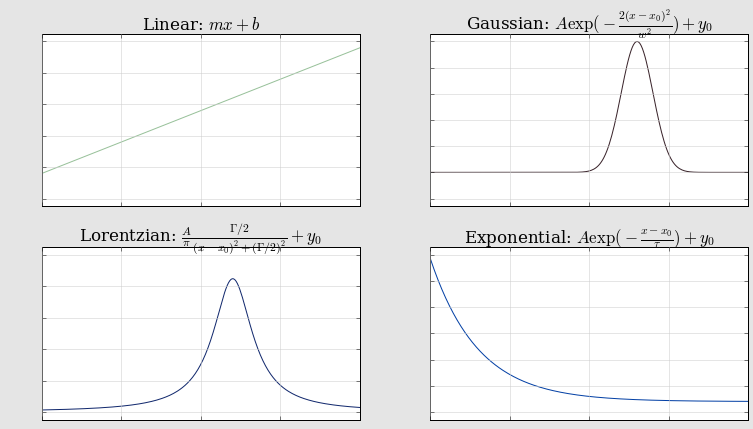
\includegraphics[width=.75\textwidth]{images/truncAllFitsHelp.png}
\caption{Truncated output of calling $\texttt{AllFits.help()}$ (with some formatting error).}
\label{fig:allfits}
\end{figure}




%%%%%%%%%%%%%%%%%%%%%%%%%%%%%%%%%%%%%%%%%%%%%%%%%%%%%%%%%%%%%%%%%%%%%%%%%%%%
%%%%				            LINES                                     %%
%%%%%%%%%%%%%%%%%%%%%%%%%%%%%%%%%%%%%%%%%%%%%%%%%%%%%%%%%%%%%%%%%%%%%%%%%%%%
\clearpage
\section{Lines}
A \texttt{Line} object is a very simple object which allows \textsc{matplotlib} to draw a line.
\begin{lstlisting}[caption={Line properties and initiation}, style=properties]
self.p           # point to draw the line
self.ls          # maybe solid '-' or dashed '--' or dotted ':'
self.vert        # bool for whether it is vertical. Default is horizontal.
self.color       # str of color
self.name        # str identifier name (maybe useless)

horLine  = Line(-34.0, '--', '#f0c8c8', 'The Minimum')
vertLine = Line(33.3,
                ls='-',
                vert=True,
                color='#99ccaa',
                name='The Maximum')
\end{lstlisting}









%%%%%%%%%%%%%%%%%%%%%%%%%%%%%%%%%%%%%%%%%%%%%%%%%%%%%%%%%%%%%%%%%%%%%%%%%%%%
%%%%				            PLOTS                                     %%
%%%%%%%%%%%%%%%%%%%%%%%%%%%%%%%%%%%%%%%%%%%%%%%%%%%%%%%%%%%%%%%%%%%%%%%%%%%%
\chapter{Plotting}


\section{Plot}
The whole point of the preceding structures is to be able to quickly add them to a plot via a list of things to plot. The general plotting function has several options which will be examined through examples. The logic in the code should be pretty easy to follow. The \texttt{Plot()} command has the following parameters:

\begin{table}[hbt]\centering
\begin{tabular}{r l l}
\textbf{listOfTraces} & \textit{list of plot objects} & The main list of \texttt{Traces}, \texttt{Waves}, \texttt{Lines}, and \texttt{Fits}. Can be a single item.  \\
\textbf{title} & \textit{str} & Plot title at top of figure  \\
\textbf{xlabel} & \textit{str} & Plot x-axis label \\
\textbf{ylabel} & \textit{str} & Plot y-axis label \\
\textbf{xlog} & \textit{bool} & Set to \textit{True} for log scale along x-axis \\
\textbf{ylog} & \textit{bool} & Set to \textit{True} for log scale along y-axis \\
\textbf{xlim} & \textit{(float, float) or None} & Manual x-axis range of form \textit{(min, max)} \\
\textbf{ylim} & \textit{(float, float) or None} & Manual y-axis range of form \textit{(min, max)}\\
\textbf{gridlines} & \textit{bool} & Set to \textit{False} to hide gridlines\\
\textbf{legend} & \textit{bool or (str, [])} & \textit{False} to hide; or \textit{("upper left", [trace, numbers, to, label])} \\
\textbf{fc} & \textit{str} & Background color of figure\\
\textbf{fs} & \textit{(float, float0)} & The \textit{(width, height)} of the image in inches\\
\textbf{dpi} & \textit{int} & Pixels per inch (default is 80)\\
\end{tabular}
\end{table}

The procedure for figure creation is currently: create the \textsc{matplotlib} figure, add gridlines, add one plot axis object, set up axis scales, convert \texttt{Waves} to \texttt{Traces}, plot all \texttt{Traces} and \texttt{Fits}, plot error bars for traces with error bars, plot all \texttt{Lines}, set title, labels, and legends. An example:

\begin{lstlisting}[caption=Using Plot()]
Plot([pts1, pts2, fit3, fit1, fit2, line1, line2],
     title='Gauss/Lor Fit Test',
     xlabel='Time (ms)',
     ylabel='Frequency (MHz)',
     xlog=False,
     ylog=True,
     xlim=[0, 10],
     gridlines=True,
     fc='#e9e9cc',
     fs=(6.0, 6.0),
     dpi=80)
\end{lstlisting}

Note that you can use LaTeX in the title and labels, but you will need to enter math mode, and inside of strings, you should double-escape everything so newline ($\backslash$n), tab ($\backslash$t), and other characters aren't replaced. For example: \texttt{xlabel='\$$\backslash\backslash$tau\$ (ms)'}.

\subsection{Colormaps}
A colormap changes point color based on $f(z)$, where the $zwave$ array needs to be stored in the $ywave$'s $clist$ property. Then the trace has to have the \textit{cmapstr} set to a valid color map string (see Fig. \ref{fig:colormaps}). Color maps are automatically scaled, so you have to deal with that yourself.
\begin{lstlisting}[caption=Error Bars on Trace After Creation]
colormask = [0, 0, 1, 1, .6, 1, 0, 0, 0, 1, .6, 1]
pts = TL.Wave([0, 1, 2, 6, 4, 3, 7, 5, 12, 2, 3, 5], name='MyWave', clist=colormask)
trace = TL.Trace(pts, cmapstr='plasma')
TL.Plot(trace, title="Color wave test")
\end{lstlisting}

\begin{figure}[hb]
\vspace{1cm}
\centering
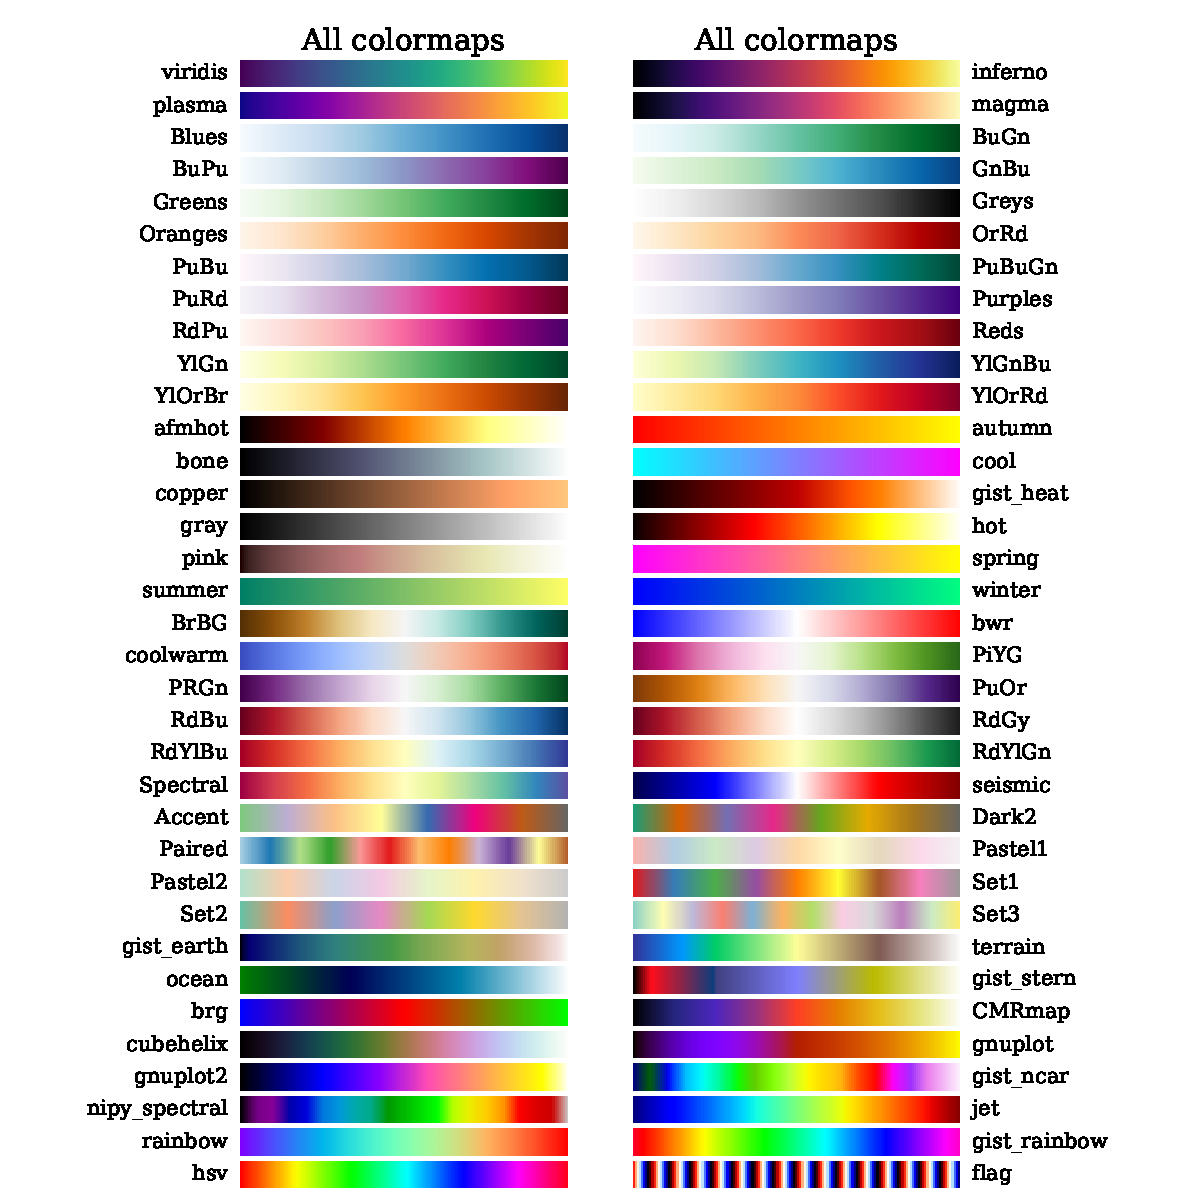
\includegraphics[width=.7\textwidth]{images/colormaps.pdf}
\caption{Default colormaps.}
\label{fig:colormaps}
\end{figure}



%%%%%%%%%%%%%%%%%%%%%%%%%%%%%%%%%%%%%%%%%%%%%%%%%%%%
%             Chapter Two: Data In                 %
%%%%%%%%%%%%%%%%%%%%%%%%%%%%%%%%%%%%%%%%%%%%%%%%%%%%
\chapter{Importing Data}\label{chap:data}
Importing data is handled through the fairly versatile \textsc{NumPy} \texttt{genfromtxt()} function. 

\section{Datasets}
The \texttt{Dataset} object is mostly a 2D numpy array $\mathcal{D}$ with some metadata, created as a result of importing a data file of rows of different points, columns of different fields. The default ordering has element $\mathcal{D}$\texttt{[i][j]} for row \texttt{i} and column \texttt{j}, but this can be transposed using the \texttt{unpack=True} parameter. Note that for a \texttt{Dataset} that contains both strings and floats, a numpy \textit{structured array} is created, and this cannot be indexed numerically except by row. Instead, \textit{headers} can be used to reference a column of interest by name. For example, suppose our data set looks like:
\begin{lstlisting}[caption=Example data contents of a .txt file]
time   AI0    GenFit1   StrVar  ...   AOM1
1.00   0.01   0.01E-3    NaN    ...    5.0
1.01   0.02   0.00E-3    NaN    ...    5.0
1.02   0.01   0.01E-3    NaN    ...    0.0
                    ...
5.00   0.01   3.14E-1    NaN    ...    0.0          
\end{lstlisting}
Importing this (either with the TSV or Datalog import functions) will create a structured array because of the "NaN" column, allowing access to the first point ($time=1.00$) with \texttt{data[0]} or access to all \textit{AI0} points through \texttt{data['AI0']}. But we cannot hope to use \texttt{data[:, 0]} or anything to get column 0 because a structured array cannot be indexed in this manner. If the data contained in the file is entirely numeric, a regular, indexable 2D array is created (still compatible with header strings).

Finally, \texttt{Waves} can be attached to \texttt{Datasets}, see the \hyperref[sec:attachwave]{next section}. The \texttt{Dataset} object structure is (see file for arguments that may go into \texttt{genfromtxt}):
\begin{lstlisting}[caption={Dataset structure}, style=properties]
self.data       # np.array from np.genfromtext()
self.name       # string identifier
self.filename   # string filename with extension
self.folder     # string of last folder (eg the date)
self.rows       # number of "data points"
self.cols       # number of "data fields"
self.headers    # column headers (in numpy, called "names")
self.isDatalog  # boolean for whether file was Master VI datalog
\end{lstlisting}


\clearpage
\subsection*{Importing Datasets}
Slightly specialized functions for importing common datasets are detailed here.
\subsubsection*{\textbf{importDatalog}({\color{args}[Rb style Datalogs from Master VI]})}


\begin{lstlisting}[caption=importDatalog]
importDatalog(filename,      # automatically appends "_XYGraphDataLog0.txt"
              name='First Dataset',
              headers=True,  # automatic from LabVIEW
              skip_header=0, # use all data points
              skip_footer=0,
              usecols=[],    # import all columns
              unpack=True,   # transpose data
              max_rows=0)    # use all data points
\end{lstlisting}


\subsubsection*{\textbf{importTimeTrace}({\color{args}[Rb style AI Time Traces from Master VI]})}
Imports 7 column AI trace file and automatically names them AI0 through AI6.
\begin{lstlisting}[caption=importTimeTrace]
importTimeTrace(filename,
                name='',
                skip_header=3, # three metadata lines for Igor
                skip_footer=3, # three metadata lines for Igor
                usecols=[],    # import all AI traces
                unpack=True,   # transpose data
                max_rows=0)    # use all data points
\end{lstlisting}


\subsubsection*{\textbf{importAIPoints}({\color{args}[Sr style AI log file]})}
Creates columns for time (first column) and AI7 through AI0 (from columns $2, 4, ..., 16$).
\begin{lstlisting}[caption=importAIPoints]
importAIPoints(filename,
               name='',
               headers=False, # will be automatic, but ["could", "overwrite", "here"]
               skip_header=0, # use all points
               skip_footer=3, # use all points
               unpack=True,   # transpose data
               max_rows=0)    # use all points
\end{lstlisting}


\subsubsection*{\textbf{importCSV}({\color{args}[Regular comma-separated table]})}
\begin{lstlisting}[caption=importCSV]
importCSV(filename,
          name='',
          headers=False, # no column names, but ["could", "set", "here"]
          skip_header=0, # use all points
          skip_footer=0, # use all points
          usecols=[],    # use all columns
          unpack=True,   # transpose data
          max_rows=0):   # use all points
\end{lstlisting}

\subsubsection*{\textbf{importTSV}({\color{args}[Regular tab-separated table]})}
\begin{lstlisting}[caption=importTSV]
importTSV(filename,
          name='',
          headers=False, # no column names, but ["could", "set", "here"]
          skip_header=0, # use all points
          skip_footer=0, # use all points
          usecols=[],    # use all columns
          unpack=True,   # transpose data
          max_rows=0):   # use all points
\end{lstlisting}



\end{document}